\documentclass[12pt, a4paper]{article}

\usepackage{multicol}
\usepackage{geometry}
\usepackage{setspace}
\usepackage{CJKutf8}
\usepackage{amsmath}
\usepackage{listings}
\usepackage{graphicx}

\title{
    \textbf{Report Title} \\
    \large Report Subtitle \\
    \small Tracy Liu
    \author Tracy Liu
    \date{}
}

\geometry{a4paper,left=2cm,right=2cm,top=2.8cm,bottom=3.2cm}
\setlength{\columnsep}{1cm}
\setlength{\baselineskip}{100pt}
\linespread{1.2}
\graphicspath{ {./images/} }

\begin{document}
    \begin{CJK*}{UTF8}{bsmi}

    % title
    \begin{center}
        \LARGE\textbf{2019 Fall Introduction to Operating Systems} \\
        \large Homework 3 \\
        \small 0616015 劉姿利 \\
    \end{center}

    % \begin{multicols*}{2}

    % contents
    \section{Briefly describe the design for the sort and merge function and the thread management in the multi-thread program.}
        \subsection{Sort}
            Brute-force bubble sort.

        \subsection{Merge}
            Two-pointer sorting.

        \subsection{Thread Management}
        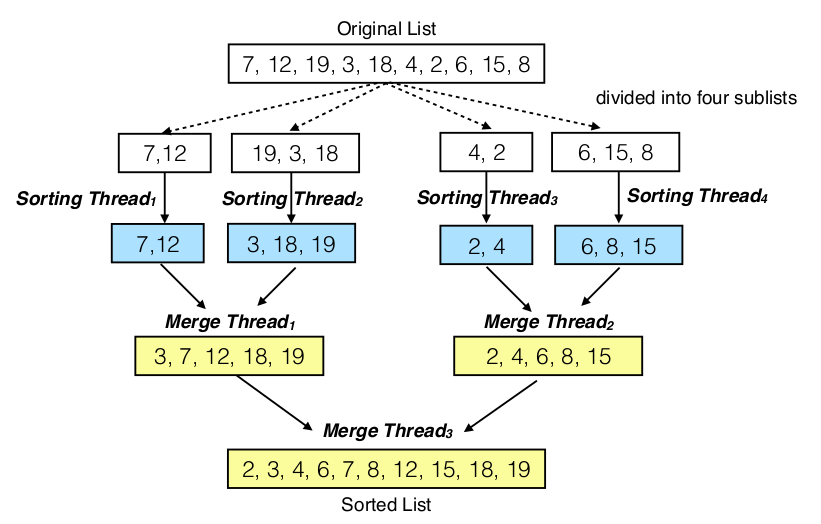
\includegraphics{threads_graph.png}
        \begin{itemize}
        \item Let each thread be either sorting\_thread or merge\_thread.
        \item For each sorting\_thread, just simple creat it and execute.
        \item For each merge\_thread, we have first wait for other 2 threads before execution.
            \begin{itemize}
            \item merge\_thread\_1 waits for sorting\_thread\_1 and sorting\_thread\_2.
            \item merge\_thread\_2 waits for sorting\_thread\_3 and sorting\_thread\_4.
            \item merge\_thread\_3 waits for merge\_thread\_1 and merge\_thread\_2.
            \end{itemize}
        \end{itemize}

        \subsubsection{Waiting Design for Merge\_threads}
            I pass the thread indexes to wait for by passing a structure S.
\begin{lstlisting}[language=C++]
void *_merge(void* data) {
    S* ptr = (S*)data;
    int id1 = ptr->id1;
    int id2 = ptr->id2;

    pthread_join(id[id1] ,NULL);
    pthread_join(id[id2] ,NULL);

    ...
}
\end{lstlisting}

    \section{Show the thread information screenshot while running the single-thread/multi-thread program.}
        \subsection{Single-thread}
            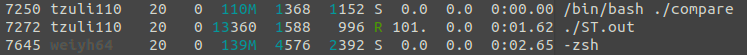
\includegraphics{st_threads.png}
        \subsection{Multi-thread}
            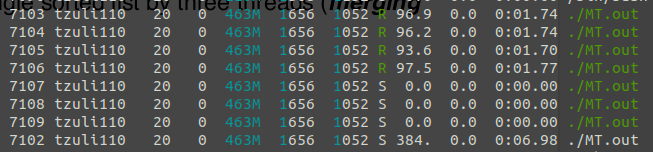
\includegraphics{mt_threads.png}


    \section{Show the time speedup between single-thread and multi-thread.}
        \subsection{Single-thread}
            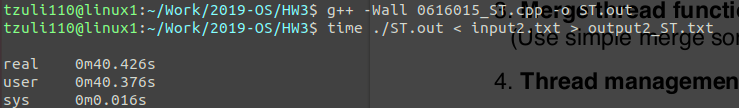
\includegraphics{st_time.png}
        \subsection{Multi-thread}
            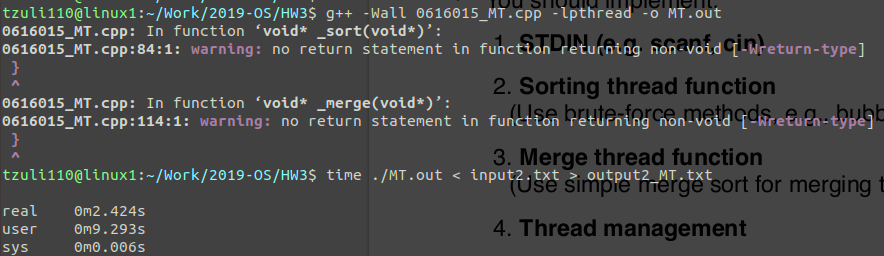
\includegraphics{mt_time.png}

    \section{What I learned from doing homework 3.}
        \begin{itemize}
        \item How to use pthread api.
        \item How to check the number of threads by using htop.
        \item How to use stucture and type conversion to pass arguments into threads.
        \end{itemize}

    % \end{multicols*}
    \end{CJK*}
\end{document}
